\documentclass[conference]{IEEEtran}

\usepackage{enumerate}
\usepackage{enumitem}
\setenumerate[1]{itemsep=0pt,partopsep=0pt,parsep=\parskip,topsep=2pt}
\setitemize[1]{itemsep=0pt,partopsep=0pt,parsep=\parskip,topsep=2pt}
\setdescription{itemsep=0pt,partopsep=0pt,parsep=\parskip,topsep=2pt}

\usepackage{longtable}
\usepackage{rotating}
\usepackage{multirow}
%\usepackage[table]{xcolor}	%for color of table cell
\usepackage{diagbox}		%for head of table

%\usepackage[tight,footnotesize]{subfigure}

\usepackage{listings}
\usepackage{color}

%\usepackage{caption}
\usepackage[noend]{algpseudocode}
\usepackage{algorithm}
\algnewcommand{\LineComment}[1]{\State \(\triangleright\) #1}

\usepackage{amsmath}
\usepackage{amsthm}
\usepackage{multirow}
%\usepackage[amsmath,thmmarks]{ntheorem}

\usepackage{empheq}
\usepackage{xcolor}
\usepackage{graphicx}
\definecolor{hellmagenta}{rgb}{1,0.75,0.9}		%for color of equations
\definecolor{hellcyan}{rgb}{0.75,1,0.9}
\definecolor{hellgelb}{rgb}{1,1,0.8}
\definecolor{colKeys}{rgb}{0,0,1}
\definecolor{colIdentifier}{rgb}{0,0,0}
\definecolor{colComments}{rgb}{1,0,0}
\definecolor{colString}{rgb}{0,0.5,0}
\definecolor{darkyellow}{rgb}{1,0.9,0}

\usepackage{amssymb}
\usepackage{stfloats}
%\usepackage[square, comma, sort&compress, numbers]{natbib}
\usepackage{mathrsfs}
\usepackage{subfigure}

\usepackage{lipsum}
\usepackage{lmodern}
\usepackage{tcolorbox}
\usepackage[linewidth=1pt]{mdframed}

%\usepackage[colorlinks,
%            linkcolor=red,
%            anchorcolor=blue,
%            citecolor=green]{hyperref}

%\usepackage[citecolor=black]{hyperref}
\usepackage{url}
\usepackage{array}
\usepackage{fancyhdr}
\usepackage{booktabs} % For formal tables
\usepackage{textcomp}

\def\BibTeX{{\rm B\kern-.05em{\sc i\kern-.025em b}\kern-.08em
		T\kern-.1667em\lower.7ex\hbox{E}\kern-.125emX}}

\begin{document}

\title{A Statistical Analysis on Recent Housing Data}

\author{
    \IEEEauthorblockN{Matthew Grohotolski, Alexander Waskiewicz}
    \IEEEauthorblockA{Elizabethtown College
    \\\{$GrohotolskiM$, $WaskiewiczA$\}@etown.edu}
}


\maketitle

\begin{abstract}

The purpose of this paper is to identify which variables have the largest influence on house value in the United States and to create a multiple linear regression model to predict house value. Using the 2019 data from IPUMS, we found that age of structure, metropolitan status, number of bedrooms, log value of property tax, and state all have significant effect on the dependent house value variable. State and property tax were two of the most significant predictors within the model. 

These results indicate possible correlation between location and house value as states and counties within those states have varying property taxes based on population size and density in the region. Age of structure was also a good predictor of home value but we believe that it could be skewed in more wealthy areas where older built homes could be renovated and upgraded. This could introduce bias into the reporting of home value as the owner gave an estimate of what they believe their house is worth. Since the housing market is constantly changing with increasing inflation from COVID-19, it is important that more research is conducted to test for other variables that could affect home price to make extrapolation into the future more accurate. 



\end{abstract}


\section{Introduction}
\label{sec:intro}


\subsection{Background}
House values in the United States are constantly shifting due to outside political and economic factors that the public does not have control of. Being able to predict house values in this ever changing market is important for home buyers across the country who are looking for the best price on a home. Having a complete understanding of the variables that affect house value will aid home buyers in assessing what their needs and wants are during this process.


\subsection{Data}
The data utilized is extracted from the IPUMS USA database from a survey conducted in 2019 by Integrated Public Use Microdata Series. IPUMS USA is a website and database that provides access to samples of the American population from sixteen different federal censuses, the American Community Surveys of 2000 to the present and from the Puerto Rican Community Surveys from 2005 to the present.\cite{IPUMS} A random sample of 100,000 units were selected from the original data for the analysis. Of the 17 predictor variables examined in the original data, 5 were used in the regression analysis and model building to predict the response variable of house value; all of which are described below. The other 12 that were omitted were either not of interest in predicting house value or did not have measurable values for the purposes of this study. 



\subsection{Variables}
\indent \textbf{State} which is described by the name "STATEFIP", reports the state in which the house was located in alphabetical order. This geographic variable includes all states and the District of Columbia as well as groupings of states which totals to 62 possible values for this explanatory variable in the original data set.\cite{IPUMS} The variables used in the random sample study only included 51 categorical variables which consisted of all the states and the District of Columbia which were represented by the various state abbreviations.


\indent \textbf{Metropolitan status} which is described by the name "METRO", indicates whether the household resided within a metropolitan area and, households in metropolitan areas, whether the household resided within or outside of a central city. This geographic variable includes 5 possible values in the original data set.\cite{IPUMS} For the study, 4 of those categorical variables were used as there were no values of "Metropolitan status indeterminable" within the 100,000 units.


\indent \textbf{Annual property taxes} which is described by the name "PROPTX99", reports the household's total real estate tax costs for the previous year. The total tax includes state, local, and any other taxes. Respondents reported the full amount of taxes including mortgage payments, delinquent payments, and if they were paid by another party. This economic variable includes 70 values, all of which are represented by an interval of property tax ranging from $50.00$ to $1000.00$ intervals in the original data set.\cite{IPUMS} With the intention of creating a simpler model, the 70 variables were condensed into 11 categorical variables represented by the median of a $1,000.00$ interval; $500.00$, $1,500.00$, $2,500.00$ e.t.c.. We renamed this variable "LNPROPTX" after taking the natural log of the property tax value to reduce variability.


\indent \textbf{Age of structure} which is described by the name "BUILTYR2", reports the decade in which the structure was built. This dwelling characteristic variable has 24 values which range from homes being built in 1939 or before to being built in 2019 in the original data set. For this study, all 100,000 randomly selected homes were built in 2005 or after which creates 14 quantitative variables.\cite{IPUMS} It was not necessary to study houses built before 2005 as the population of interest is only in recently built homes. Making the "BUILTYR" variable quantitative will give a simpler model. The years after 2005 were represented by values of 10 through 24. These values were re-coded into years 2005 to 2019.


\indent \textbf{Number of bedrooms} which is described by the name "BEDROOMS", reports the number of bedrooms within the housing unit. This dwelling characteristic variable has 22 possible values with x-1 being the number of bedrooms represented by each value (x) in the original data set. The data in this study did not include any units with greater than 8 bedrooms so there are 9 categorical variables for bedroom.\cite{IPUMS} The variable values for bedrooms were all transformed into x-1 values to make this a quantitative representation of the number of bedrooms.


\indent \textbf{House value} which is described by the name "VALUEH", reports the value of the housing units in contemporary dollars. This value was collected based on the home owners opinion of the value of their home at the time of the survey. House value is a continuous variable from houses built in 2008 and on. There are 65 possible values in the original data set that are represented by intervals in which a homeowners property tax would be included in.\cite{IPUMS} For this study, the categorical intervals were reverted into quantitative values that the owners originally priced their homes at. The variable was renamed "LNVALUE" after the natural log was taken to reduce variability. This will allow for analysis to become simpler when testing variables that may have a significant effect on house value.


\subsection{Exploratory Data Analysis}

Fig. \ref{figure:state_counts} shows an overview of the house count in each state from the simple random sample (SRS) of 100,000 data entries.

\begin{figure}[h!]
	\centering
	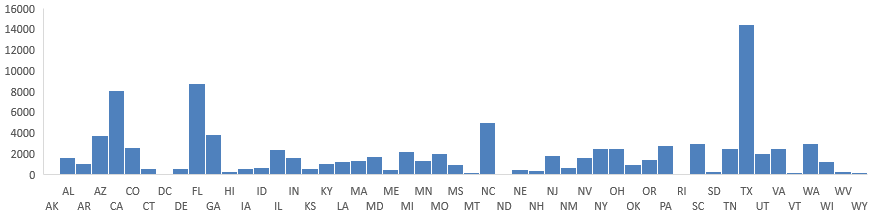
\includegraphics[width=3.5in]{./fig/State_Counts.PNG}
	\caption{Count of Houses per State}
	\label{figure:state_counts}
\end{figure}

Fig. \ref{figure:year_counts} shows a plot of the count of houses built by year from the SRS.

\begin{figure}[h!]
	\centering
	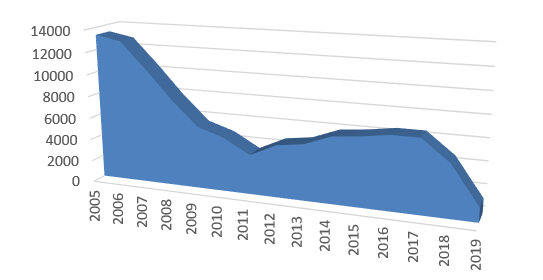
\includegraphics[width=3.5in]{./fig/Year_Counts.PNG}
	\caption{Count of Houses Built by Year}
	\label{figure:year_counts}
\end{figure}

Fig. \ref{figure:PROPTX_Comparison} shows a plot comparing the distribution of average property tax in each state with the log distribution of average property tax in each state from the SRS.

\begin{figure}[h!]
	\centering
	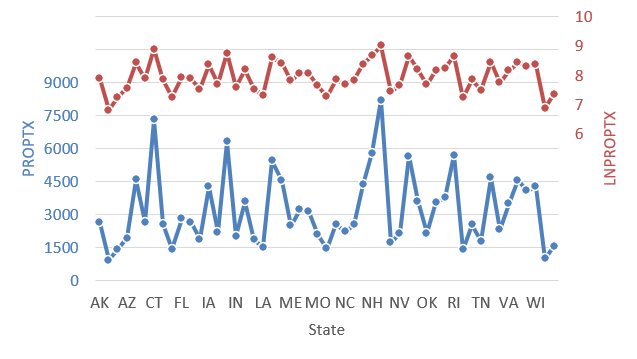
\includegraphics[width=3.5in]{./fig/PROPTX_Comparison.PNG}
	\caption{PROPTX vs. LNPROPTX}
	\label{figure:PROPTX_Comparison}
\end{figure}

Fig \ref{figure:VALUE_Comparison} shows a plot comparing the distribution of average home values in each state with the log distribution of average home values in each state from the SRS.

\begin{figure}[h!]
	\centering
	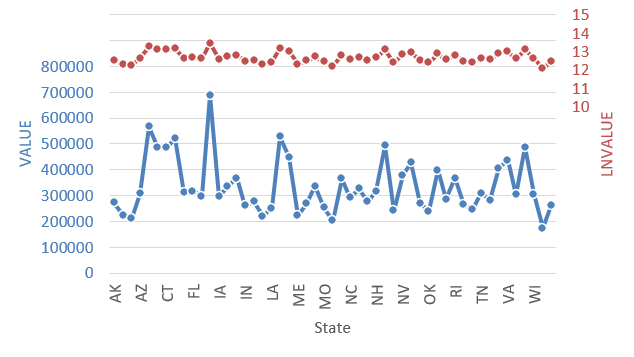
\includegraphics[width=3.5in]{./fig/VALUE_Comparison.PNG}
	\caption{VALUE vs. LNVALUE}
	\label{figure:VALUE_Comparison}
\end{figure}

\section{Methods}
\label{sec:methods}


A multiple linear regression model was used with house value as the response variable. We tested 5 possible models by using the same 5 explanatory variables examined in the \textbf{variables} section but with different selection procedures and criteria. We took the natural log of property tax and predicted value in order to increase the r-squared value while decreasing variance. This means that we will be predicting the log value of a house with the final model. The step wise procedure was used for the first three models where the different selection criteria values of BIC, CP Mallow, and p-value were used. For the other two models, we took the selection criteria that had the best fit from the first three models (p-value) and used it with the forward selection procedure and then the backward selection procedure. We chose this process as a way to standardize selection procedure and predictor variables which allowed for comparison of the multiple model's ability to predict house price. 



\input{results}
\section{Discussion}
\label{sec:disc}

\subsection{Significant Variables}
Of the 8 predictor variables utilized in the model, age of structure, state (Texas), number of bedrooms, and log of property tax were the most significant predictors of home value in the model with each variable mentioned below having a p-value of less than 0.0001. All intercepts are in terms of predicted log house values. To convert these log coefficients to U.S. dollar amounts, use this equation. \[ USD=10^x \] where x is a log coefficient.

Age of structure had an intercept value of 0.009527. As the age of structure becomes newer by 1 year, the average predicted log home value increases by 0.009527 holding all other variables constant.

The state of Texas had an intercept value of -0.851144. The average predicted log home value for a house in Texas is 0.851144 less than a house in Pennsylvania holding all other variables constant.

Number of bedrooms had an intercept value of 0.135463. For every 1 bedroom increase, the average predicted log home value increases by 0.135463 holding all other variables constant.

Log of property tax had an intercept of 0.560288. For each 1 unit increase in log of property tax, the average predicted log home value increases by 0.560288 holding all other variables constant.

The coefficients for the significant predictor variables are located are located in a GitHub file due to spacing conflicts with this report. View References section for the link.\cite{github}.

\subsection{Limitations}
A few of the variables were challenging to represent originally which made the model more complex and confusing to interpret. One of these variables, age of structure had to be made into a quantitative variable in order to obtain the assumption plots within a reasonable amount of processing time in SAS. This limits our ability to interpret the effect on house price that each year has individually and our ability to compare years with our intended year of interest of 2019. With this variable, extrapolation is very dangerous for years outside of the range 2005 to 2019 as there are confounding variables that could affect home value such as economic prosperity, inflation rates, and general value of the U.S. dollar.

It is also important to mention that the years of 2008 and 2009 could include multiple outliers because these observations were collected directly following the Great Recession in late 2007 from the housing market crash. We expect these housing values to be extremely lower compared to 2005, 2006, and 2007 which would make the predicted model hard to use during the years in which the country was recovering from the market crash. More research should be completed to find if variables such as employment status of owners or mortgage value are more significant for predicting home value during this recession.

\bibliographystyle{IEEEtran.bst}
\bibliography{refs}

\end{document}
